\documentclass[a4paper]{article}


\usepackage{alphabeta} 
\usepackage{enumitem} 
\usepackage{mathtools}
\usepackage{amsmath, amssymb} 
\usepackage{amsthm}
\usepackage{cancel} 
\usepackage[margin=0.70in]{geometry} 
\geometry{left=3cm,right=3cm,top=2.4cm,bottom=2.4cm}	%the page geometry as defined, A4=210x297mm
\usepackage{graphicx}
\usepackage{wrapfig}
\usepackage[center]{caption}
\usepackage{textcomp}
\usepackage{tabto}
\usepackage{layout}
\usepackage{bm}
\usepackage{minipage-marginpar}
\usepackage[dvipsnames]{xcolor}
\usepackage{hyperref}
\usepackage{dutchcal}
\usepackage{derivative}
\usepackage{esint}
%\usepackage{biblatex}
\usepackage{subcaption}
\usepackage{booktabs}\usepackage{derivative}
\usepackage[flushleft]{threeparttable}
\usepackage[capbesideposition=outside,capbesidesep=quad]{floatrow}
\usepackage{derivative}
\usepackage[thinc]{esdiff}
\usepackage{lipsum}
\usepackage{arydshln}
\usepackage{physics}
%%RENEW

\newtheorem{problem}{Άσκηση}
\newtheorem*{solution*}{Λύση}
\newtheorem{definition}{Ορισμός}[subsection]
\newtheorem{properties}{Ιδιότητες}[subsection]
\newtheorem{theorem}{Θεώρημα}[subsection]
\newtheorem{protash}{Πρόταση}[subsection]
\newtheorem{porisma}{Πόρισμα}[subsection]
\newtheorem{lemma}{Λήμμα}[subsection]
\newtheorem*{prooof}{Απόδειξη}
\newtheorem*{notes}{Παρατηρήσεις}
\newtheorem*{note}{Παρατήρηση}
\newtheorem*{app}{Εφαρμογή} 
\newtheorem*{example}{Παράδειγμα}
\newtheorem*{examples}{Παραδείγματα}


\newcommand\numberthis{\addtocounter{equation}{1}\tag{\theequation}}
%\renewcommand{\labelenumi}{\roman{enumi}}
\newcommand{\approxtext}[1]{\ensuremath{\stackrel{\text{#1}}{\approx}}}
\renewcommand{\figurename}{Εικόνα.}
\renewcommand{\tablename}{Πίνακας.}
%\renewcommand\refname{New References Header}
\renewcommand*\contentsname{Περιεχόμενα}
%\DeclareDerivative{\odv}{\mathrm{d}}


\begin{document}
\begin{titlepage}			%makes a title page. Remember to change the author, CID, username and group number to what is appropriate for you!
	\centering
	{\scshape\LARGE Εθνικό Μετσόβιο Πολυτεχνείο\par}
	{\scshape \LARGE Σ.Ε.Μ.Φ.Ε.\par}
	\vspace{1cm}
	{\huge\bfseries Παραμαγνητικός Συντονισμός Πυρήνων (NMR)\par}
	\vspace{1cm}
	{\Large\itshape Θωμόπουλος Σπύρος\par}		%remember to change these!
	
	%		{\large Group \@group\unskip\strut\par}
	{\large spyros.thomop@gmail.com/ ge19042@mail.ntua.gr\par \hfill \\}% 		%remember to change these!
	\vspace{1cm}
	{\large Ημερμονηνία Παράδοσης 23/05/2022\par}
\end{titlepage}

\subsection*{Σκοπός}
	Ο σκοπός της εν λόγω εργαστηριακής άσκησης είναι η μελέτη του παραμαγνητικού συντονισμού πυρήνων και η μέτρηση του συντελεστή g των πρωτονίων.
	
\subsection*{Θεωρητικά Στοιχεία}
	Ο παραμαγνητικός συντονισμός σχετίζεται γενικά με τον συντονισμό της κίνησης που εκτελεί ένα μαγνητικό δίπολο με ένα εξωτερικά μεταβαλλόμενο μαγνητικό πεδίο. Στην περίπτωσή μας συγκεκριμένα θα μελετήσουμε το φαινόμενο του Παραμαγνητικού Συντονισμού Πυρήνων. Η αλληλεπίδραση του πυρήνα με το μαγνητικό πεδίο θα δίνεται από την Hamiltonian
		\begin{align*}\label{1}
			H_B = -\textbf{μ}_N\cdot\textbf{B} =& -\gamma_N \hbar\textbf{J}_N\cdot\textbf{B} \Rightarrow\\
			    =& g_N \beta_N \textbf{J}_N\cdot \textbf{B}\numberthis
		\end{align*}

όπου $\gamma_N =\frac{e}{2m_N}$ ο γυρομαγνητικός λόγος, $\textbf{μ}_N = \frac{e}{2m_N}\textbf{J}_N = \gamma_N\textbf{J}_N $ και $\beta_N$ η πυρηνική μαγνητόνη.

	\subsubsection*{1ο Βήμα}
		Αν βάλουμε ισχυρό σταθερό μαγνητικό πεδίο $\textbf{B}_0=B_0\hat{z}$, τότε θα έχουμε ότι το μαγνητικό δίπολο θα εκτελέσει μεταπτωτική κίνηση γύρω από τον άξονα $\hat{z}$ με συγκεκριμένη συχνότητα, την συχνότητα Larmor: 
		\begin{align}\label{2}
			\Omega_L = \gamma_NB_0 
		\end{align}
		
Μέχρι εδώ δεν γίνεται λόγος για συντονισμό. Απλά τοποθετώντας ένα μαγνητικό δίπολο όπως ο πυρήνας σε ομογενές μαγνητικό πεδίο, παρατηρούμε πως θα εκτελέσει μεταπτωτική κίνηση. Εδώ μπορεί να σημειωθεί πως περιμένουμε ότι η συχνότητα Larmor στον NMR θα είναι αρκετές τάξεις μικρότερη από του EPR καθώς η μάζα μπαίνει στον παρονομαστή και η μάζα του πυρήνα θα είναι φυσικά μεγαλύτερη απ' του ηλεκτρονίου.
	
	\subsubsection*{2ο Βήμα}		
		Τώρα τοποθετούμε ένα κυκλικά πολωμένο μαγνητικό πεδίο κάθετα στο αρχικό $\textbf{B}_0$, με συχνότητα περιστροφής $\omega$, που έχει μορφή:
		\begin{align}
			\textbf{B} = \hat{x} Bcos\omega t - \hat{y}Bsin\omega t
		\end{align}
	Τώρα η Hamiltonian γράφεται ως 
		\begin{align*}\label{3}
			H =& H_0 + H_B = -\textbf{μ}\cdot\textbf{B}_0 - \textbf{μ}\cdot\textbf{B} =\Rightarrow \\ 
			  =& -\gamma_N B_0 \frac{\hbar}{2} \sigma_z -\gamma_N B\frac{\hbar}{2}\left(\sigma_x cos\omega t-\sigma_y sin\omega t\right)	\Rightarrow\\
			  =& -\gamma_N B_0 \frac{\hbar}{2}\smqty(\pmat{3}) -\gamma_N B\frac{\hbar}{2}\left( \smqty(\pmat{1})cos\omega t -\smqty(\pmat{2})sin\omega t  \right) \Rightarrow \\ 
			  =& \begin{pmatrix}-\hbar\Omega_L/2&0\\0&\hbar\Omega_L/2\end{pmatrix} - \gamma B\frac{\hbar}{2}\begin{pmatrix}0&e^{i\omega t}\\e^{-i\omega t}&0\end{pmatrix} \Rightarrow\\
			  =&\begin{pmatrix}-E_L& E_Be^{i\omega t} \\E_Be^{-i\omega t}&E_L\end{pmatrix} \numberthis
		\end{align*}			
		όπου $E_L= \hbar \Omega_L/2 $ και $E_B=-\gamma B\hbar/2$. Τώρα η επίλυση της χρονοεξαρτημένης εξίσωση Schrodinger για την παραπάνω Hamiltonian, $i\hbar\pdv{}{t}|\psi\rangle = H|\psi\rangle$ , θα δώσει μία συχνότητα περιστροφής ίση με
		\begin{align}\label{4}
			\Omega_R (\omega) =& \sqrt{\left(\frac{\omega - \Omega_L}{2}\right)^2 +\left( \frac{\gamma_N B}{2} \right)^2}	\xRightarrow{(\ref{1})} \\
			=& \frac{\gamma_N}{2}\sqrt{\left(B_0-\frac{\omega}{\gamma_N}\right)^2 +B^2}		
		\end{align}
	
	Τώρα παρατηρούμε ότι όταν $\omega = \Omega_L$, δηλαδή όταν το πεδίο περιστρέφεται μαζί με το δίπολο, τότε η ένταση του στατικού πεδίου στο περιστρεφόμενο σύστημα αναφοράς του \textbf{B} θα είναι μηδέν και το μονο πεδίο που θα δρα στον πυρήνα θα είναι το \textbf{B}. Τότε, η πιθανότητα για να μεταβεί το δίπολο από την κατάσταση που είναι παράλληλη με το πεδίο στην αντιπαράλληλη είναι η μέγιστη και μάλιστα ίση με ένα. Δηλαδή, σίγουρα θα αντιστραφεί, όπως προκύπτει από την λύση της εξίσωσης Schrodinger.
	
	Αν τώρα $\omega\neq\Omega_L$ δεν έχουμε σίγουρη αλλαγή κατάστασης προς την αντιπαράλληλη, αλλά όταν βρισκόμαστε σε μία περιοχή κοντά στην $\Omega_L$ δημιουργείται ένα μέγιστο τόσο στην πιθανότητα μετάβασης όσο και στην καμπύλη παραμαγνητικών απωλειών. Οι μαγνητικές απώλειες προκύπτουν διότι κατά την αντιστροφή, το μαγνητικό δίπολο θα πρέπει να προσλάβει ενέργεια.
	%\\
	
	Επιπλέον, αν θεωρήσουμε ότι οι πυρήνες μας έχουν μαγνητικό αρθμό $m_J=\pm1/2$, τότε η κβαντομηχανική επιβάλλει ότι οι μεταβάσεις της ενέργειας θα είναι 
	\begin{align}\label{5}
		\Delta E = \hbar\omega =\gamma_N\hbar B_0 \Rightarrow \omega = \gamma_N B_0 \equiv\Omega_L
	\end{align}


Ακόμη, πρέπει να επισημανθεί το ότι τα μαγνητικά πεδία που ''νιώθουν'' εν τέλει οι πυρήνες δεν είναι τα ίδια με τα εφαρμοζόμενα καθώς επηρεάζονται και από τα τοπικά μαγνητικά πεδία που δημιουργούν τα ηλεκτρόνια.
	\vspace{-0.3cm}
	\subsubsection*{Κορεσμός}
Καθώς αυξάνουμε την ένταση του μεταβαλλόμενου μαγνητικού πεδίου, από μία τιμή και έπειτα παρατηρείται η μείωση του σήματος NMR. Το σήμα NMR πρόκειται για την τιμή της μαγνητική επιδεκτικότητας συναρτήσει του χρόνου αποκατάστασης ισορροπίας $T_1,T_2$ των διπόλων στις διευθύνσεις $\hat{z}$ και $\hat{x},\hat{y}$ και γι' αυτό θα περιμέναμε να αυξάνεται με την αύξηση του πλάτους του μαγνητικού πεδίου.
	
	Έστω $N_1$ και $N_2$ είναι οι πληθυσμοί των διπόλων που είναι προσανατολισμένοι αντίστοιχα παράλληλα και αντιπαράλληλα με το στατικό πεδίο. Τότε, όταν το μεταβαλλόμενο πεδίο έχει μικρή ένταση, οι θερμικές κινήσεις των διπόλων τα επαναφέρουν στην αρχική τους κατάσταση άρα η διαφορά $N_1-N_2$ παραμένει σταθερή.  Αυξάνοντας περεταίρω το πεδίο μειώνεται η διαφορά των πληθυσμών και ολοένα αυξανόμενος αριθμός διπόλων αναστρέφεται αντιπαράλληλα απ΄ το πεδίο, δηλαδή τα δίπολα (πυρήνες) αναστρέφονται με γρηγορότερο ρυθμό απ' ότι τα επαναφέρει η θερμοκρασία στην αρχική τους κατάσταση.
	\vspace{-0.3cm}
\subsection*{Πειραματική Διάταξη}

 Ο στόχος εδώ είναι να καταγράψουμε την καμπύλη συντονισμού, δηλαδή την μαγνητική επιδεκτικότητας συναρτήσει της συχνότητας της γεννήτριας $f_0$ και του παράγοντα μεταβολής του στατικού πεδίου και έπειτα να αντλήσουμε από αυτή τα στοιχεία που μας χρειάζονται. 
 
 Αυτό θα το πετύχουμε κρατώντας σταθερή την συχνότητα $f_0$ μίας γεννήτριας που καθορίζει την συχνότητα περιστροφής του πεδίου (στην πραγματικότητα έχουμε αντικαταστήσει το περιστρεφόμενο πεδίο με γραμμικά πολωμένο καθώς αυτό είναι πιό εύκολο να παραχθεί πειραματικά) και αλλάζοντας την ένταση του στατικού πεδίου, εως ότου η συχνότητα Larmor των διπόλων (\ref{2}) γίνει ίση με την συχνότητα της γεννήτριας. Τότε αν αυξομειώνουμε το στατικό πεδίο $\textbf{B}_0$ θα εμφανιστεί η χαρακτηριστική καμπύλη συναρτήσει του μαγνητικού πεδίου. 
 
 Το κυριότερο μέρος της διάταξης είναι το παρακάτω κύκλωμα Γέφυρας 
 
 \begin{figure}[h!]
 	\centering
 	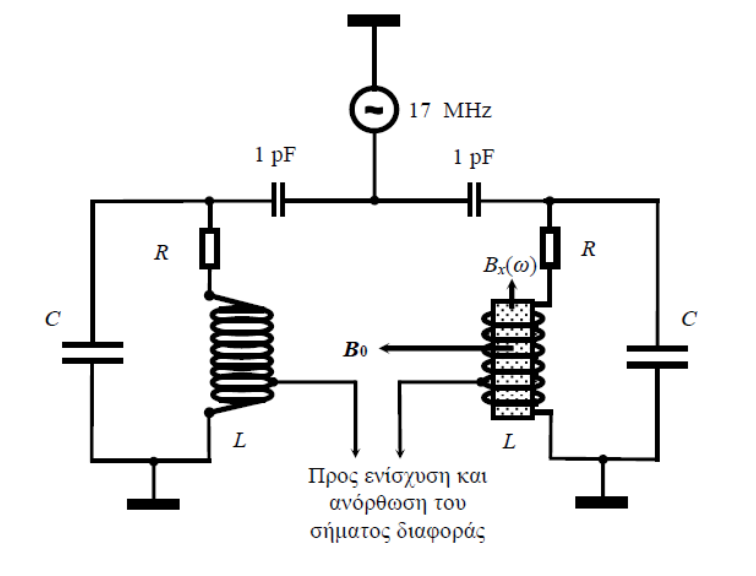
\includegraphics[scale=0.42]{im1.png}
 	\caption{Κύκλωμα Γέφυρας}
 	\label{im1}
 \end{figure}

Η γέφυρα αποτελείται από δύο όμοια και παράλληλα κυκλώματα RLC που ταλαντώνονται με την συχνότητα $f_0\sim10-20MHz$ της γεννήτριας και τα κυκλώματα βρίσκονται σε κατάσταση ισορροπίας οι τάσεις στα δύο πηνία είναι ίσες. Αν τώρα τοποθετήσουμε στο εσωτερικό του ενός πηνίου ένα μαγνητικό υλικό, τότε μεταβάλλεται η αυτεπαγωγή του και έτσι διαταράσσεται η ισορροπία μεταξύ των δύο κυκλωμάτων. Έτσι έχουμε διαφορετικές τάσεις στις άκρες των πηνίων και αυτή η διαφορά δυναμικού που αρχικά είναι της τάξης των $\mu V$ ενισχύεται και όταν έχουμε συντονισμό μεγιστοποιείται

\subsection*{Πειραματική Διαδικασία - Επεξεργασία Μετρήσεων}

	Στο πείραμά μας θα παρατηρήσουμε τον συντονισμό NMR στους πυρήνες του υδρογόνου της γλυκερίνης η οποία είναι τοποθετημένη σε μία γυάλινη αμπούλα.
	Αφού θέσουμε σε λειτουργία τα στοιχεία του κυκλώματος μεταβάλλουμε το ρεύμα στα πηνία από $2.8-3.5Α$ με βήμα 0.1Α και καταγράφουμε τις τιμές της συχνότητας και του μαγνητικού πεδίου το οποίο μετράμε με ένα μαγνητόμετρο
	\begin{table}[h!]
		\centering
		\begin{tabular}{r|r|r}
			I(A) & $B(\pm2mT)$ & $f(\pm0.01MHz)$ \\\hline\hline
			2.8& 379& 16.31\\
			2.9& 388& 16.71\\
			3.0& 396& 17.32\\
			3.1& 405& 17.49\\
			3.2& 414& 18.83\\
			3.3& 422& 18.17\\
			3.4& 430& 18.52\\
			3.5& 437& 18.82
		\end{tabular}
		\caption{ }
		\label{mat1}
	\end{table}
	
	Εφαρμόζοντας την μέθοδο των ελχίστων τετραγώνων για τα μεγέθη f-B, προκείπτει η παρακάτω ευθεία (έχω επιβάλλει να είναι της μορφής $y=ax$):
		\begin{figure}[h!]
			\centering
			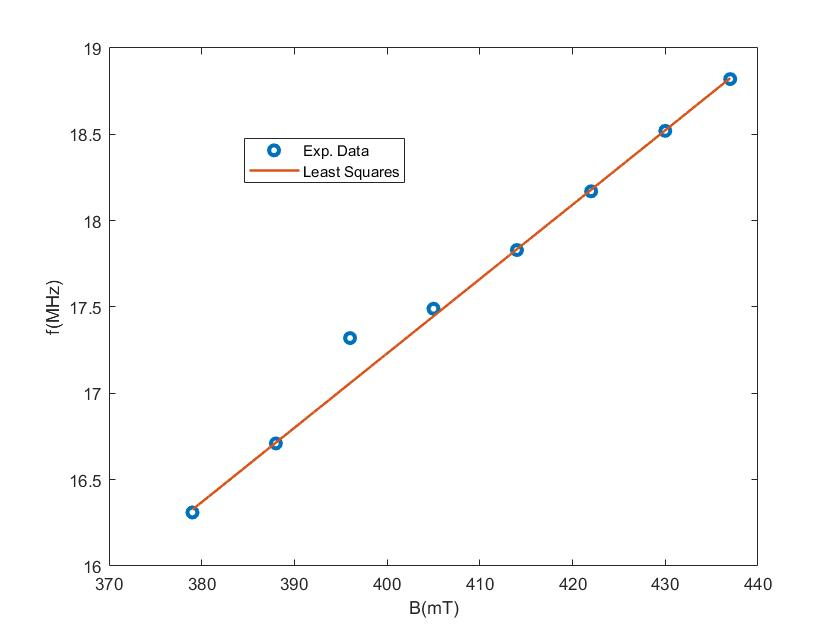
\includegraphics[scale=0.4]{plot1.jpg}
			\caption{ }
			\label{im2}
		\end{figure}
		
Στην μέθοδο δεν έχω συμπεριλάβει την τρίτη τιμη καθώς ξεφεύγει κατά πολύ από τις υπόλοιπες. Η κλίση προκύπτει $A = (431\pm1)\times10^5Hz/T$.%\footnotemark	.

%\footnotetext{Το σφάλμα προκύπτει ως $\delta A=\delta A_{στατ.}+\delta A_{οργ}$, όπου $\delta A_{στατ.}= 1\times10^{-5}$ και $\delta A_{οργ}=A(\gamma_f+\gamma_B)= A(\Delta B/B + \Delta f/f) = 431\times10^{-5}(0.1422+0.1419) =  $}

Τώρα χρησιμοποιώντας την σχέση 	
	\begin{align*}
		f= \underbrace{g\frac{\beta_N}{h}}_{A}B
	\end{align*}
		όπου $\beta_N=5.051\times10^{-27}J/T$ θα υπολογίσω τον γυρομαγνητικό παράγοντα 
	\begin{align*}
		A = f\frac{\beta_N}{h}\Rightarrow g = \frac{Ah}{\beta_N} \Rightarrow \boxed{g= 5.65\pm0.02}
	\end{align*}			
		η οποία έχει σχετικό σφάλμα με την θεωρητική $\sim1.5\%$, το οποίο είναι σχετικά μικρό.
\subsection*{Συμπεράσματα}


Εν τέλει τα αποτελέσματά μας είναι ικανοποιητικά, καθώς η τιμή του g που υπολογίστηκε είναι αρκούντως κοντά στην αναμενόμενη, με σχετικό σφάλμα $\sim1.5\%$.





\end{document}



